\documentclass[10pt]{article}
\PassOptionsToPackage{hyphens}{url}
\usepackage{hyperref}
\usepackage[margin=0.75in]{geometry}

\usepackage{textcomp}
\usepackage{color}
\usepackage{graphicx}
\definecolor{pblue}{rgb}{0.13,0.13,1}
\definecolor{pgreen}{rgb}{0,0.5,0}
\definecolor{pred}{rgb}{0.9,0,0}
\definecolor{pgrey}{rgb}{0.46,0.45,0.48}

\usepackage{listings}
\lstdefinestyle{term}{language=bash,
  columns=fullflexible,
  showspaces=false,
  showtabs=false,
  breaklines=true,
  showstringspaces=false,
  tabsize=2,
  breakatwhitespace=true,
  commentstyle=\color{pgreen},
  keywordstyle=\color{pblue},
  stringstyle=\color{pred},
  numbers=left,
  stepnumber=1,
  basicstyle=\small\ttfamily,
  frame=single,
  moredelim=[il][\textcolor{pgrey}]{$$},
  moredelim=[is][\textcolor{pgrey}]{\%\%}{\%\%},
  upquote=true
}
\lstdefinestyle{sh}{language=bash,
  columns=fullflexible,
  showspaces=false,
  showtabs=false,
  breaklines=true,
  showstringspaces=false,
  tabsize=2,
  breakatwhitespace=true,
  commentstyle=\color{pgreen},
  keywordstyle=\color{pblue},
  stringstyle=\color{pred},
  numbers=left,
  stepnumber=1,
  basicstyle=\small\ttfamily,
  frame=single,
  moredelim=[il][\textcolor{pgrey}]{$$},
  moredelim=[is][\textcolor{pgrey}]{\%\%}{\%\%},
  upquote=true
}

\lstdefinestyle{py}{language=python,
  columns=fullflexible,
  showspaces=false,
  showtabs=false,
  breaklines=true,
  showstringspaces=false,
  tabsize=2,
  breakatwhitespace=true,
  commentstyle=\color{pgreen},
  keywordstyle=\color{pblue},
  stringstyle=\color{pred},
  numbers=left,
  stepnumber=1,
  basicstyle=\small\ttfamily,
  frame=single,
  moredelim=[il][\textcolor{pgrey}]{$$},
  moredelim=[is][\textcolor{pgrey}]{\%\%}{\%\%},
  upquote=true
}

\title{\textbf{Week 09} \\
\LARGE Apache2 and Flask \\
\Large Making a Professional Webserver}
\author{
	Melvyn Ian Drag
}
\date{\today}


\begin{document}
\maketitle

\begin{abstract}
Last class we took a look at the toy `SimpleHTTPServer' in Python3. Tonight we'll use a real website backend - Flask - and we'll server content on a real server - Apache2. As before, we'll make \textbf{GET} and \textbf{POST} requests using the command line tool cURL.
\end{abstract}


\section{What's a Webserver?}
The term is overloaded. A server is a computer, connected to a network, that
other computers can access. It also refers to software than responds to client
requests. 2 Weeks ago we saw a Postgres server. This week we'll make an Apache2
webserver. So The word can refer to hardware ( the computer itself ) or software
(the software that responds to client requests).

\section{What's Flask?}
Flask is what is called a \textbf{Back End Web Framework}. Its a bunch of code
that some one smarter than us already wrote to handle GET and POST requests in a
really pretty way. It's amazing that this stuff is free. You're about to get a
professional website online in a few minutes thanks to a bunch of generous smart
people giving us this Flask code.

There are other backend frameworks. In Python lots of people use Django. In Java
lots of folks use Play, Spring, and a bunch of others.

\section{What's a REST API? What's JSON? }
REST is an acronym for a beautiful but complex
topic. For the rest of the lecture just understand that if you get JSON from a
webserver, you're probably talking to it's REST API. We saw a REST API last week
when you made requests with curl to api.github.com and it responded with some
stuff that looked like:
 
\begin{verbatim}
{
	"name": {
		"first": "melvyn",
		"last": "drag"
	},
	"profession": "programmer",
	"favoriteLanguages": ["C++", "Python"]
}
\end{verbatim}

That's what JSON looks like, and it's fantastic stuff.

Too many acronyms in CS, right?

\begin{itemize}
\item JSON - JavaScript Object Notation
\item API - Application Programming Interface
\item REST - REpresentational State Transfer
\end{itemize}

Scary stuff to look at, but we'll take a peek today.

\section{What we'll do today}
Today we'll bring a real website online. Last week we made a trivial website
with Python's SimpleHTTPServer, but today we're going to use a real,
professional-grade server ( Apache2 ) and a real backend web framework ( Flask
). There are other servers like NGINX and there are other backend webframeworks
like Django, Play, Spring, Ruby on Rails, etc., I've just chosen this pair
because it's the easiest to code of the few things I know. Deploying a Spring
app on an NGINX server is probably as simple as what I've prepared for you
today, and if you want to be a web developer then you should totally go research
how to do it!

\begin{figure}[h]
  \centering
    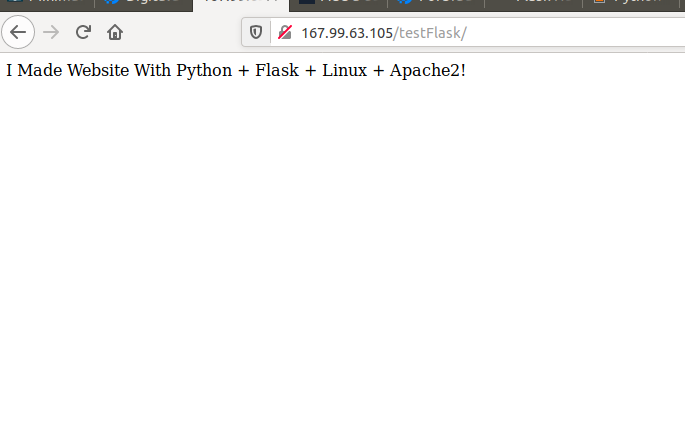
\includegraphics[width=0.8\textwidth]{Exercise1Success.png}
  \caption{A website running on my server at IP address
http://167.99.63.105/testFlask/ . This is the first website we will build
together today. It will run on Linux using Python, Flask and Apache2}
\label{fig:firstsite}
\end{figure}


Plan for today:
\begin{enumerate}
\item Example 1: Boring website that just returns text. See figure
\ref{fig:firstsite}
\item Example 2: Little more interesting website that returns HTML
\item Example 3: Even more interesting website that returns JSON.
\end{enumerate}

\section{Setting up server}
So let's begin building our Flask + Apache2 website. Get a debian 10 server on
digital ocean. Then run these commands:

\begin{lstlisting}[style=term, caption=configure your server, label=lst:install]
root@machine$ apt update
root@machine$ apt install git apache2 libapache2-mod-wsgi-py3 python3-dev
python3-pip curl
# so now we have git for the class code
# apache2 for the webserver
# python3 for the backend framework
# curl for making HTTP requests
root@machine$ pip3 install flask flask-restful
# now that we have python3 we can install flask.
root@machine$ service apache2 status
# should report that apache2 is running
root@machine$ curl localhost
# lots of data
root@machine$ curl localhost > curlResponse.html
# dump the data to a file so it's easier to look through
root@machine$ less curlResponse.html # look through, verify you have the default apache page. That means the server is running.
root@machine$ curl ipinfo.io/ip # get your server ip address
\end{lstlisting}

Open a browser on a laptop or computer. Go to the server ip address, make sure the server is running. You should see the same default apache page you saw with curl localhost. But now you are looking at it through a browser on a different machine ( you ran curl on the webserver itself ).

\begin{figure}[h]
  \centering
    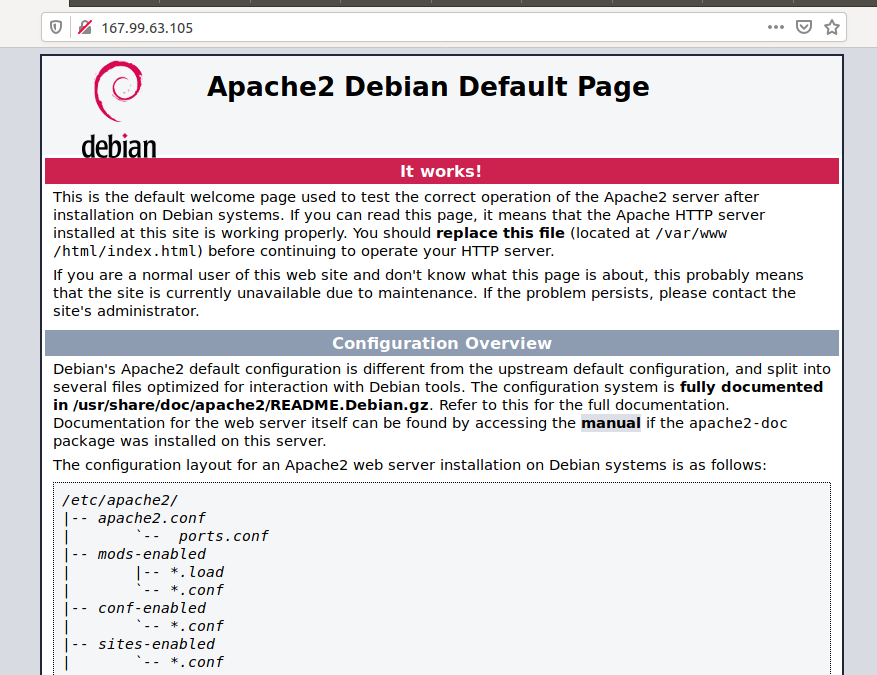
\includegraphics[width=0.8\textwidth]{defaultApache.png}
  \caption{default webpage provided by a fresh Apache2 install}
	\label{fig:default}
\end{figure}

So we've installed all the software we need! That was easy. Now we can build a little website and then connect the website code to the apache server we just installed and activated.

{\Large \color{red} Warning! Make sure you have succeeded in this first task. If
you haven't, you won't be able to do the rest of the exercises. If you can see
the default Apache webpage, then continue on. }

Congratulations!! You've set up your first Apache webserver! Wasn't that easy???
Linux is good.

\section{Example 1: Deploying Your First Flask Application}
The first thing we need to do is create a non root user for managing this stuff. We'll give the user sudo permission for the few root things we need to do to bring the website online. I've created user `webdeveloper'. You should do the same so you can copy and paste the code I've provided. If you create a different username, you'll need to make the minor modifications to make everyting match up.

\begin{lstlisting}[style=term]
root@machine$ adduser webdeveloper
root@machine$ usermod -a -G sudo webdeveloper
root@machine$ su - webdeveloper
webdeveloper@machine$ cd ~
webdeveloper@machine$ git clone https://github.com/melvyniandrag/LinuxClassRepo.git
webdeveloper@machine$ cp -r
LinuxClassRepo/Lectures/Week10_Apache2_And_Flask/Example1/ExampleFlask ExampleFlask
webdeveloper@machine$ ls
LinuxClassRepo ExampleFlask
webdeveloper@machine$ ls ExampleFlask
__init__.py my_flask_app.py my_flask_app.wsgi
\end{lstlisting}

Let's take a quick minute to inspect these files. These files will be confusing
to you, but they're important. I'm just going to show them to you on the off
chance that you're curiosity gets piqued so you can go out and learn more.

\subsection{\_\_init\_\_.py}
What is this empty file doing here? You'll need to go find a good Python book or
online tutorial if you want to know. There's no time to discuss what this is
now.

\begin{lstlisting}[style=term, caption=Notice that \_\_init\_\_.py is empty]
webdeveloper@machine$ pwd 
/home/webdeveloper/ExampleFlask
webdeveloper@machine$ cat __init__.py
webdeveloper@machine$ 
\end{lstlisting}

\subsection{my\_flask\_app.py}\label{sec:example1python}

This is the Python code for our website. It contains a single function
\textit{hello()} that is available at the route "/". So, assume we have a
domain name \textit{www.mydomain.com} for this little website. To access the
\textit{hello()} function, we have to go to \textit{www.mydomain.com/} ( note
the slash at the end ). We could put other routes like \textit{/otherroute}, and
indeed we will do this in the next exercise. Be patient!

\lstinputlisting[style=sh, caption=Flask is such a cool framework. Look how
short the code is!]{Example1/ExampleFlask/my_flask_app.py}


\subsection{my\_flask\_app.wsgi}
\label{sec:example1wsgi}
I believe we already said that python apps dont run on the internet by default.
You need a "little something extra" to make it work. That something extra is
WSGI and you'll see that we already installed it at the beginning of the lecture
when you installed \textit{libapache2-mod-wsgi-py3}. This library lets python3
apps run on your webserver. Anyway, this .wsgi file contains some configuration
stuff to get the website working. You'll need to study Flask in depth to
understand what this file is and how I created it.

\lstinputlisting[style=sh, caption=Deploying Flask apps on Linux servers is
easy! This configuration file is so short and sweet!]{Example1/ExampleFlask/my_flask_app.wsgi}


\section{Connect Flask to Apache2}
Now we need to wire up our Flask application to the Apache webserver software. You will need to know your machine's ip address.

\begin{lstlisting}[style=term, caption=Run this command to get your server's ip
address., label=lst:ip]
webdeveloper@machine$ curl ipinfo.io/ip
192.34.61.215
\end{lstlisting}

Now you need to get a configuration file for the website into the \textit{/etc}
directory. The configuratin file is provided in the class repo in
Lectures/Week10*/Example1. Just copy it over.

\begin{lstlisting}[style=term, caption=Get the configuration file]
webdeveloper@machine$ sudo su -
root@machine$ cp \
/home/webdeveloper/LinuxClassRepo/Lectures/Week10/Example1/ExampleFlask.conf \
/etc/apache2/sites-available/ExampleFlask.conf
\end{lstlisting}

Now you must change the ip address in this file to the ip address of your
server. Remember when we got the ip address above in listing \ref{lst:ip}?
Here's what the file looks like. Don't forget to change the ip address! This is
the configuration file used by Apache2 to run your website.

\lstinputlisting[style=sh, caption=Apache2 configuration file, label=lst:example1conf]{Example1/ExampleFlask.conf}

\subsection{Turn on and Test the Website}
Alright then, let's do this! Run these commands as the user `webdeveloper'
\begin{lstlisting}[style=term]
webdeveloper@machine$ sudo a2ensite ExampleFlask
webdeveloper@machine$ sudo a2enmod wsgi
webdeveloper@machine$ sudo service apache2 restart
\end{lstlisting}

Then, open a browser on your laptop or the NJCU PC in front of you and go to 

\begin{center}
\textit{my.ip.addr.ess/testFlask}
\end{center}

You should see a message saying you've made your first website with Linux,
flask, apache and python, just like I showed you at the beginning of lecture in
figure \ref{fig:firstsite} . You can share the link to show off your website to your friends and family! You could now also go to godaddy or namecheap, buy a domain name, and wire that up to your server so people can go to website.com instead of a scary looking ip address.

\subsection{Additional Considerations for Example 1}
So we have a simple flask app running on apache now. As you've probably seen by now, Linux servers are very particular about groups and permissions. I'm not sure about all of the ins and outs of the permissions for Flask and Apache. I'm showing the permisisons and groups I've set up on my machine. If you do something else I'm not sure it will work, and I don't know why it owuld be broken. We could experiment with permissions if you have something else.


I'm also not sure about all the details of the ExampleFlask.conf file. There are many options to it. I've always set mine up by scouring the internet for information and banging in what ever details I found. I hope to one day understand this file in depth, but for now all I know is how to make it work.

\begin{figure}[h]
  \centering
    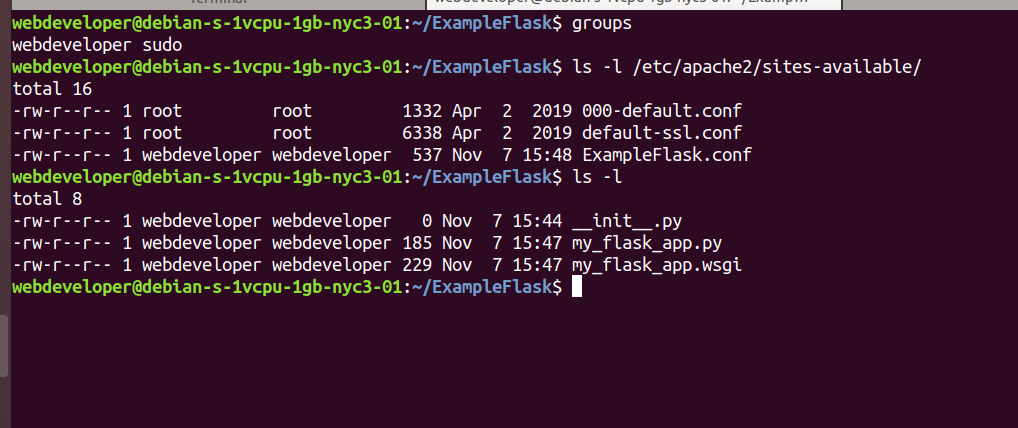
\includegraphics[width=0.8\textwidth]{groupsAndPermissions.png}
  \caption{My permissions and groups on a successful install}
\end{figure}

{\LARGE Wait for class to all be caught up and have their servers running}

\subsection{About the code for Example 1}
This isn't a Python class as we said, but I'll just mention a few things about the Python code so you get some sense of how it's working. You will see the line

\begin{lstlisting}[style=py]
@app.route("/")
def hello():
	return "some string here"
\end{lstlisting}
 
This says that when we GET the location "/" in our domain name, the webserver will respond with the return value.

But then why do we have to go to \textit{192.34.61.215/testFlask} and not just
\textit{192.34.61.215/} ( as we said in section \ref{sec:example1python} ? We
have to go to \textit{192.34.61.215/testFlask/} to see this data because in our config file we have the line

\begin{lstlisting}[style=sh]
...
WSGIScriptAlias /testFlask /home/webdeveloper/ExampleFlask/my_flask_app.wsgi
...
\end{lstlisting}

and this registers the base end point for our website as /testFlask.

The contents of the .wsgi file shown in section \ref{sec:example1wsgi} is boilerplate stuff that won't matter to you unless you want to become a serious python developer. Also, the purpose of the .wsgi file is interesting, but probably won't matter to you. Python applications can't run natively on webservers. So, about 20 years ago, some developers go together and wrote some middleware that allowds Python applications to communicate with webserver software like Apache2. The details are complicated - you can read about it if you're curious. 

\url{https://en.wikipedia.org/wiki/Web_Server_Gateway_Interface}


\section{Example2: Adding Endpoints and Serving HTML}
In the last exercise we just had our website return text - but websites
typically return either HTML ( if you're using a browser ) or JSON ( if you're
talking to the website via a REST API with a tool like curl. Let's start by
making a website that returns HTML, since it's not much harder than the last one
we set up.

Luckily for you I've prepared a simple website that returns HTML. Let's set it
up:

\begin{lstlisting}[style=term, caption=Deploying our second website]
webdeveloper@machine$ pwd
/home/webdeveloper
webdeveloper@machine$ ls
LinuxClassRepo ExampleFlask
webdeveloper@machine$ cp -r
LinuxClassRepo/Lectures/Week10_Apache2_And_Flask/Example2/ExampleFlask2
ExampleFlask2
webdeveloper@machine$ ls
LinuxClassRepo ExampleFlask ExampleFlask2
webdeveloper@machine$ ls ExampleFlask2
__init__.py my_flask_app.py my_flask_app.wsgi
\end{lstlisting}

Good, we have the new code in place. Now let's copy over the new configuration
file too.

\pagebreak

{\LARGE LISTEN!!!!}

\begin{itemize}
\item Don't forget top change the ip address in ExampleFlask.conf to the ip
address of your server.
\item Don't forget to change the ip address.
\item Change the ip address.
\item Change the ip address.
\item Change the ip address.
\end{itemize}

\pagebreak

\begin{lstlisting}[style=term, caption=Get the configuration file]
webdeveloper@machine$ sudo su -
root@machine$ cp \
/home/webdeveloper/LinuxClassRepo/Lectures/Week10/Example2/ExampleFlask.conf \
/etc/apache2/sites-available/ExampleFlask.conf
\end{lstlisting}


Also, let's delete the old default webpage config files so we don't see the
stuff we saw in figure \ref{fig:default} anymore. We don't care about the
default apache page, that was just there to let us know it installed right.

\begin{lstlisting}[style=term,caption=get rid of default site]
root@machine$ a2dissite 000-default.conf
root@machine$ rm /etc/apache2/sites-available/000-default.conf
\end{lstlisting}

Okay, good to go! Let's just restart apache and then the new site will be
active!

\begin{lstlisting}[style=term, caption=Restart the apache2 service.]
webdeveloper@machine$ sudo service apache2 restart
\end{lstlisting}

If you want to skip ahead and see what it should look like, jump ahead and look
at figure \ref{fig:sameold} and figure \ref{fig:returnshtml}.

{\Large \color{red} NOTE! Browser \textit{cache} stuff. Since we already visited
your.ip.address before, back when it was the Apache default page, your browser
may have cached that. So when you try to go to your.ip.address now, you might
still see the default page. But we disabled that thing!! How the heck is it
still coming up in our browser?? Caching. Thats how. Clear your browser cache.
On firefox you do that by hitting CTRL + F5. If that doesn't work for you use
google to figure out how. It's easy to, there will be a button to click or
something. }


\subsection{New /etc/apache2/sites-available/ExampleFlask.conf}
We've made a couple of changes to the Apache2 config file. Nothing major. 
Note that now we are serving the website at \textit{/} and not at
\textit{/testFlask}. Compare the WSGIScriptAlias line from listing
\ref{lst:example2conf} and listing \ref{lst:example1conf}. 
 
\lstinputlisting[style=sh, caption=new config file, label=lst:example2conf]{Example2/ExampleFlask.conf}

\subsection{my\_flask\_app.py}
This is interesting! Now the website has two functions in it, and two routes!
You see the same old one from Example 1, but we've added a second on that
returns HTML. This website still stinks, but we're getting somewhere! 

\lstinputlisting[style=py, caption=new Python file, label=lst:example2py]{Example2/ExampleFlask2/my_flask_app.py}

\subsection{my\_flask\_app.wsgi}
\lstinputlisting[style=py, caption=new wsgi file]{Example2/ExampleFlask2/my_flask_app.wsgi}

\subsection{\_\_init\_\_.py}
Blank as before. If you are curious, go read a Python textbook to understand what this strange file
is doing here.

\subsection{ Results }
Here are some images showing your new site in action. Check out the two routes
you created in your .py file! Here they are in the browser:

\begin{figure}[h]
  \centering
    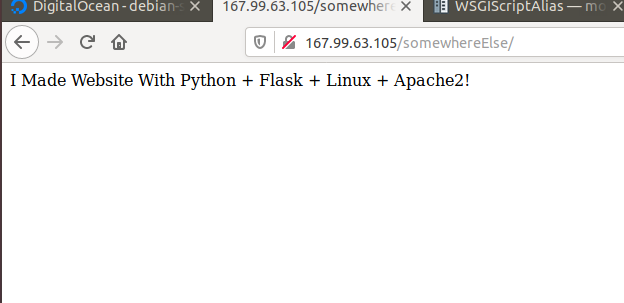
\includegraphics[width=0.8\textwidth]{somewhereElse.png}
  \caption{somewhereElse now works}
	\label{fig:sameold}
\end{figure}

\begin{figure}[h]
  \centering
    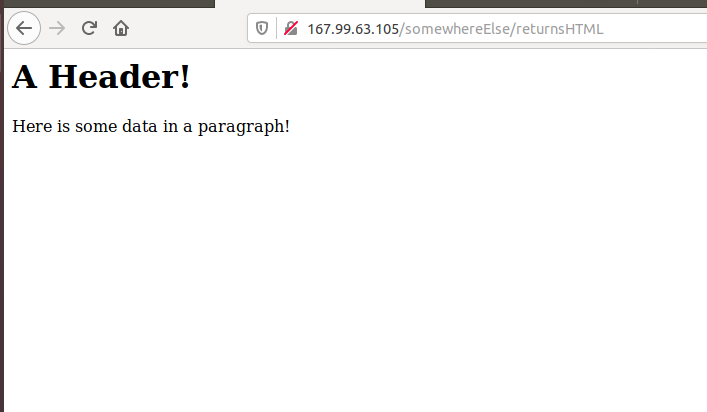
\includegraphics[width=0.8\textwidth]{somewhereElse_returnsHTML.png}
  \caption{We can now return HTML from our Flask website too!}
\label{fig:returnshtml}
\end{figure}

{\LARGE Wait for class to all be caught up and have their servers running again}

\section{Example3: A Rest API using the Flask-RESTful Library}
\subsection{Introduction}
Last week you saw a rest api in action when we talked to the github rest api.
You saw that a website returned you JSON, and not the HTML you are likely used
to receiving. When you go on amazon.com and click stuff, what you're seeing is
HTML and CSS. But when you work with a rest api (typically via curl or a simliar
tool like Postman ), you typically send and receive JSON.

What is JSON? Its a data format that looks like this:

\begin{verbatim}
{
	"name": {
		"first": "melvyn",
		"last": "drag"
	},
	"profession": "programmer",
	"favoriteLanguages": ["C++", "Python"]
}
\end{verbatim}

What's a REST API? Can REST APIs exchange other data besides JSON? 

If you're curious about this, then go find a good book or online lesson about
it! It's such interesting stuff but now is not the time.

\subsection{What websites offer REST APIs?}
A whole bunch. Github. Reddit. Twitter. Facebook. Urban dictionary. NASA. Give
it a google. Maybe you'll be bored one day and you can play with a REST api for
a new site besides github.

Today we're going to put a REST API on YOUR website.

\subsection{What's Flask-RESTful?}
It's a python library that allows you to implemet a REST api with the Flask
framework. You'll remember we installed it a long time ago as shown in listing
\ref{lst:install}

Read more here: \url{https://flask-restful.readthedocs.io/en/latest/}.

\subsection{Let's get started}
So we'll just see how to return json from a Flask application.
Same process as last time. Copy the files from Example3 to the appropriate
locations.

\begin{lstlisting}[style=term, caption=Deploying our third website]
webdeveloper@machine$ pwd
/home/webdeveloper
webdeveloper@machine$ ls
LinuxClassRepo ExampleFlask
webdeveloper@machine$ cp -r
LinuxClassRepo/Lectures/Week10_Apache2_And_Flask/Example3/ExampleFlask3
ExampleFlask3
webdeveloper@machine$ ls
LinuxClassRepo ExampleFlask ExampleFlask2 ExampleFlask3
webdeveloper@machine$ ls ExampleFlask3
__init__.py my_flask_app.py my_flask_app.wsgi
\end{lstlisting}

Good, we have the new code in place. Now let's copy over the new configuration
file too.

\begin{lstlisting}[style=term, caption=Get the configuration file for example 3]
webdeveloper@machine$ sudo su -
root@machine$ cp \
/home/webdeveloper/LinuxClassRepo/Lectures/Week10/Example3/ExampleFlask.conf \
/etc/apache2/sites-available/ExampleFlask.conf
\end{lstlisting}


Restart apache and it will work!

\begin{lstlisting}[style=term, caption=Restart the apache2 service.]
webdeveloper@machine$ sudo service apache2 restart
\end{lstlisting}


\subsection{The Flask Application: my\_flask\_app.py}
You can skim the code to see what it does. It has some code for handling the GET and POST requests. A GET request will echo back to you the entire contents of the TODOS data it's maintaining. A POST request will add to the TODOS data set. You can verify after POSTing that your data was added by sending a GET request.

\lstinputlisting[style=py]{Example3/ExampleFlask3/my_flask_app.py}

\subsection{Accessing Our REST API}
Then you can get JSON data in the browser as shown below:

\begin{figure}[h]
  \centering
    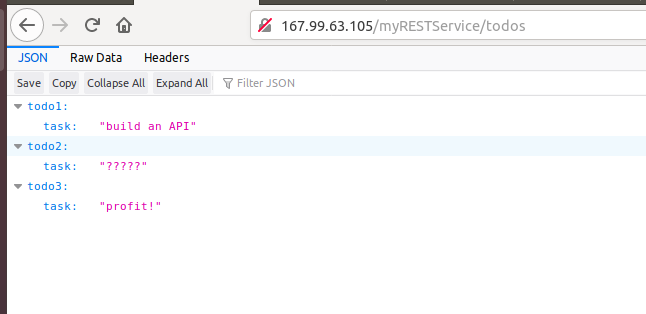
\includegraphics[width=0.8\textwidth]{restInBrowser.png}
  \caption{See some json in the browser!}
\end{figure}

Then, on your laptop, make a GET request with cURL


\begin{figure}[h]
  \centering
    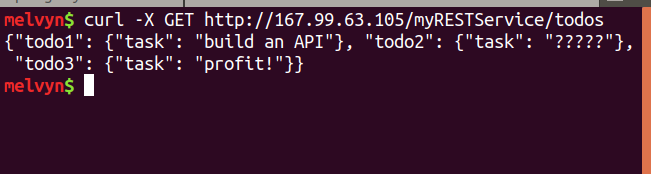
\includegraphics[width=0.8\textwidth]{curlYourAPI.png}
  \caption{Make a GET request with cURL!}
\end{figure}

And, you should also be able to make the following POST request:

\lstinputlisting[style=sh]{curlExample.sh}

And then look, after POSTing data, when you GET data you will see the data that you POSTed!

\begin{figure}[h]
  \centering
    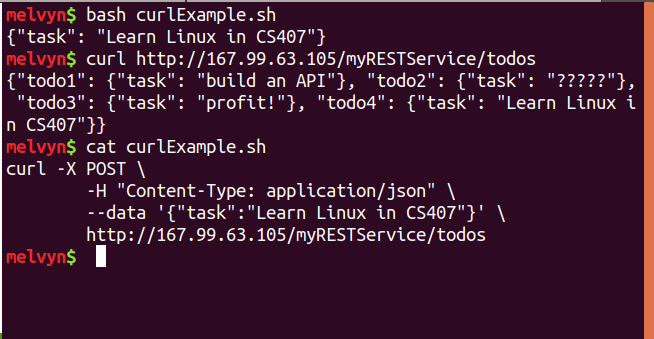
\includegraphics[width=0.8\textwidth]{addedToTODOList.png}
  \caption{POST data to your website with cURL!}
\end{figure}

\pagebreak

\section{Flask and Bigger Websites}
Typically your website code will return HTML. I've only shown you how to return HTML strings in example 2, but typically you create HTML templates and populate the template with data. Too complicated to explain, there is no time. Google 'Flask and HTML templates' if you want to know more.

NOTE if class ends early, we can do this together, but I suspect we'll be plenty busy tonight.

\section{Databases}
For your exam you set up a postgres server with some data in it. I've just shown you how to set up a Flask web application on an Apache server. And you have a good knowledge now about some linux server maintenance things. 

In the TODOList REST application we stored all of our data in a dictionary - in the real world this is not how you do it. Can you guess what you do for real websites? You use a DATABASE! You are now poised to go pick up a book on Flask and learn how to wire a database and a website backend together!

Of course we won't do that in this class, but now you have the prerequisite information to go and follow a tutorial on building websites with Flask.

\section{sed}
sed is one of the more popular command line tools. So far we know grep, vim, cat, mv, ls, etc.. sed is another one of the "big ones".

sed stands for ``stream editor" and is a simple little programming language ( or tool, depending how you want to view it ) that is used for processing text files line by line.

\subsection{What to do with sed \#1}
Sed can be used to replace all occurences of a string in a file.
See sedExamples/01.

\begin{lstlisting}[style=term]
user@machine$ cat oldFile
user@machine$ sed 's/hello//' oldFile
# will replace first occurences of 'hello' with nothing\
# note that a line with two occurences of 'hello' will only have the first occurence replaced
user@machine$ cat oldFile
# the file is not changed. sed did not overwrite the original file
user@machine$ sed 's/hello/HELLO/' oldFile
# see first occurences of hello were replaced with HELLO
\end{lstlisting}

these changes were done in place. If you want to create a new file you can do it like this

\begin{lstlisting}[style=term]
user@machine$ sed 's/hello/HELLO' <oldFile >newFile
user@machine$ sed 's/hello/HELLO' oldFile >newFile
user@machine$ sed 's/hello/HELLO' 0<oldFile >newFile
# all of the above are equivalent
\end{lstlisting}

or you can change the input file in place

\begin{lstlisting}[style=term]
sed -i  's/HELLO/hewwo/' newFile
\end{lstlisting}

the -i means `in place'.

\subsection{What to do with sed \#2}
We saw sed can do search and replace first occurence per line. It can also replace all occurrences in a file.

\begin{lstlisting}[style=term]
user@machine$ sed 's/hello/HELLO/g' oldFile
#note all occurences of hello now say HELLO
\end{lstlisting}

by adding the g after the search/replace pattern you can replace all occurences.

\subsection{What to do with sed \#3}
Sed can do regular expressions. If you want to capitalize any 'h' at the start of a line, you can do this:

\begin{lstlisting}[style=term]
user@machine$ sed 's/\(^[h]\)//' oldFile
ello world
ello world world
world hello hello world
\end{lstlisting}

\subsection{What to do with sed \#4}
You can also extract patterns. This is a weird thing that you can't always do with things like search/replace in microsoft word/excel/whatever other tools you are familiar with.

the same command as before remembers and stores the search pattern in a variable called \textbackslash1. You can do the same thing with \textbackslash2, \textbackslash3, etc for subsequent search patterns. \textbf{The search patterns are the regexs enclosed in \textbackslash( and \textbackslash)}. In the example above, my regex was looking for a line that starts with h. If you scroll down a bit youll see a regex for a line that starts with an ASCII letter.

\begin{lstlisting}[style=term]
sed 's/\(^[h]\)/\1\1\1/' oldFile
hhhello world
hhhello world world
world hello hello world
\end{lstlisting}

You may not be mentally prepared to appreciate what I've just shown you? Maybe one day you'll be trying to do a complicated search and replace task and then you'll remember sed!

Check out this interesting example too!

\begin{lstlisting}[style=term]
user@machine$ sed 's/\(^[a-zA-Z]\)/\1\1\1/' oldFile
hhhello world
hhhello world world
wwworld hello hello world
\end{lstlisting}

If I want to wrap the first letter of every line with smileys, for example, I can do this:

\begin{lstlisting}[style=term]
user@machine$ # emojis!
user@machine$ sed 's/\(^[a-zA-Z]\)/\xF0\x9F\x98\x82\1\xF0\x9F\x98\x82/' oldFile
# look what comes out! Depending on your laptop, the output will be different from the output I have as can be seen in the figure below
\end{lstlisting}


\begin{figure}[h]
  \centering
    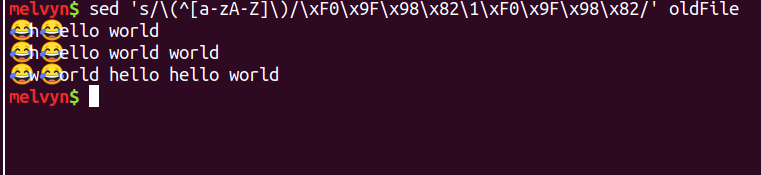
\includegraphics[width=0.8\textwidth]{mayOrMayNotWorkForYou.png}
  \caption{How the heck did he do that? If you already know, I'm very impressed}
\end{figure}

But this may or may not work on your computer, we'll talk about this in depth if there is time this semester.

\section{References}
This lecture was based on what I read  on these websites:

\url{https://www.codementor.io/abhishake/minimal-apache-configuration-for-deploying-a-flask-app-ubuntu-18-04-phu50a7ft}


There were some bugs in the tutorials above that I sorted out to make sure our lecture had a good flow.
\end{document}
